\subsection{Arsitektur yang Mengoptimalkan PostgreSQL (PGP)}

Arsitektur ini mengoptimalkan sistem dengan pola CQRS dan pola penyeimbangan beban berbasiskan antrean.

\begin{figure}[htbp]
    \centering
    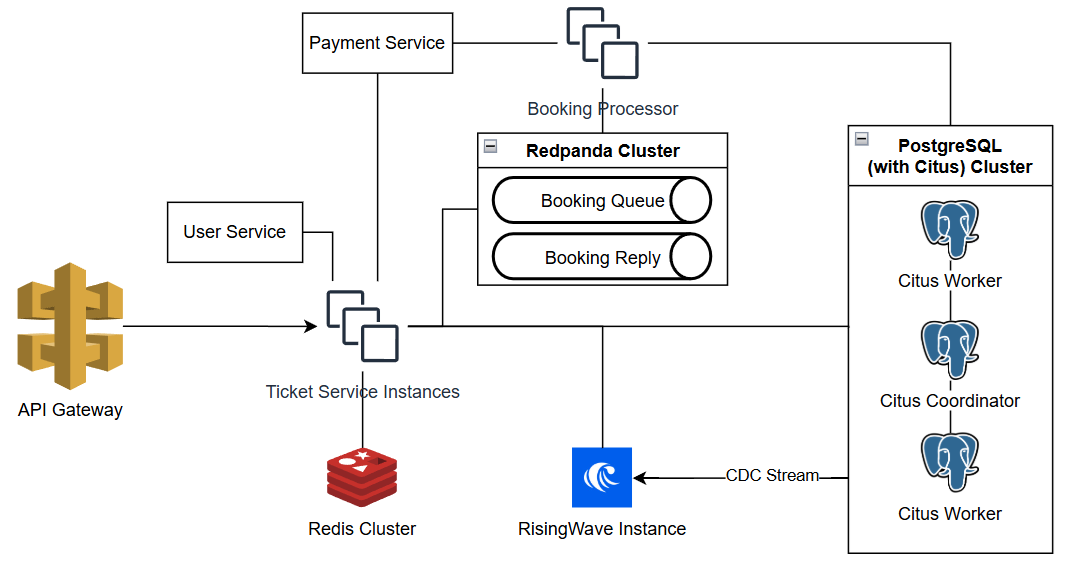
\includegraphics[width=1\textwidth]{resources/appendix/architecture-optimized.png}
    \caption{Arsitektur yang Mengoptimalkan PostgreSQL}
    \label{fig:optimized-architecture}
\end{figure}

\subsubsection{Peningkatan \textit{Throughput} PostgreSQL dengan Citus}

Penggunaan ekstensi Citus memungkinkan peningkatan \textit{throughput} dengan pendekatan \textit{scale-out}. Peningkatan ini tidak hanya pada \textit{throughput} baca, tetapi juga \textit{throughput} tulis. Hal ini dapat dicapai dengan pembagian data pada tabel berdasarkan baris, lalu setiap \textit{node} yang memegang bagian data tersebut dibuat menjadi \textit{writer}.

\textit{Sharding} berdasarkan baris ini dapat dilakukan pada tabel Seats, IssuedTicket, OrderItem, dan Orders. Entitas sisanya dapat dibuat sebagai tabel yang direplikasi ke setiap node.

\subsubsection{Penggunaan Pola Penyeimbangan Beban dengan Antrean}

Perintah pemesanan tiket (berupa \textit{command}/ \textit{event sourcing}) akan dimasukkan ke dalam antrean Redpanda terlebih dahulu. Lalu, \textit{booking processor} akan memproses permintaan secara bertahap berdasarkan kemampuan sistem. Pendekatan ini memungkinkan terjaganya stabilitas sistem ketika terdapat \textit{burst request}.

Selain itu, akan lebih baik apabila sistem dapat menolak permintaan pesanan lebih awal, seperti karena sudah ada pesanan yang sedang diproses tetapi masih belum \textit{commit}. Hal ini dapat didukung dengan penggunaan Redis untuk menyimpan \textit{uncommited data} yang akan digunakan untuk menolak permintaan pesanan lebih awal.

\begin{figure}[htbp]
    \centering
    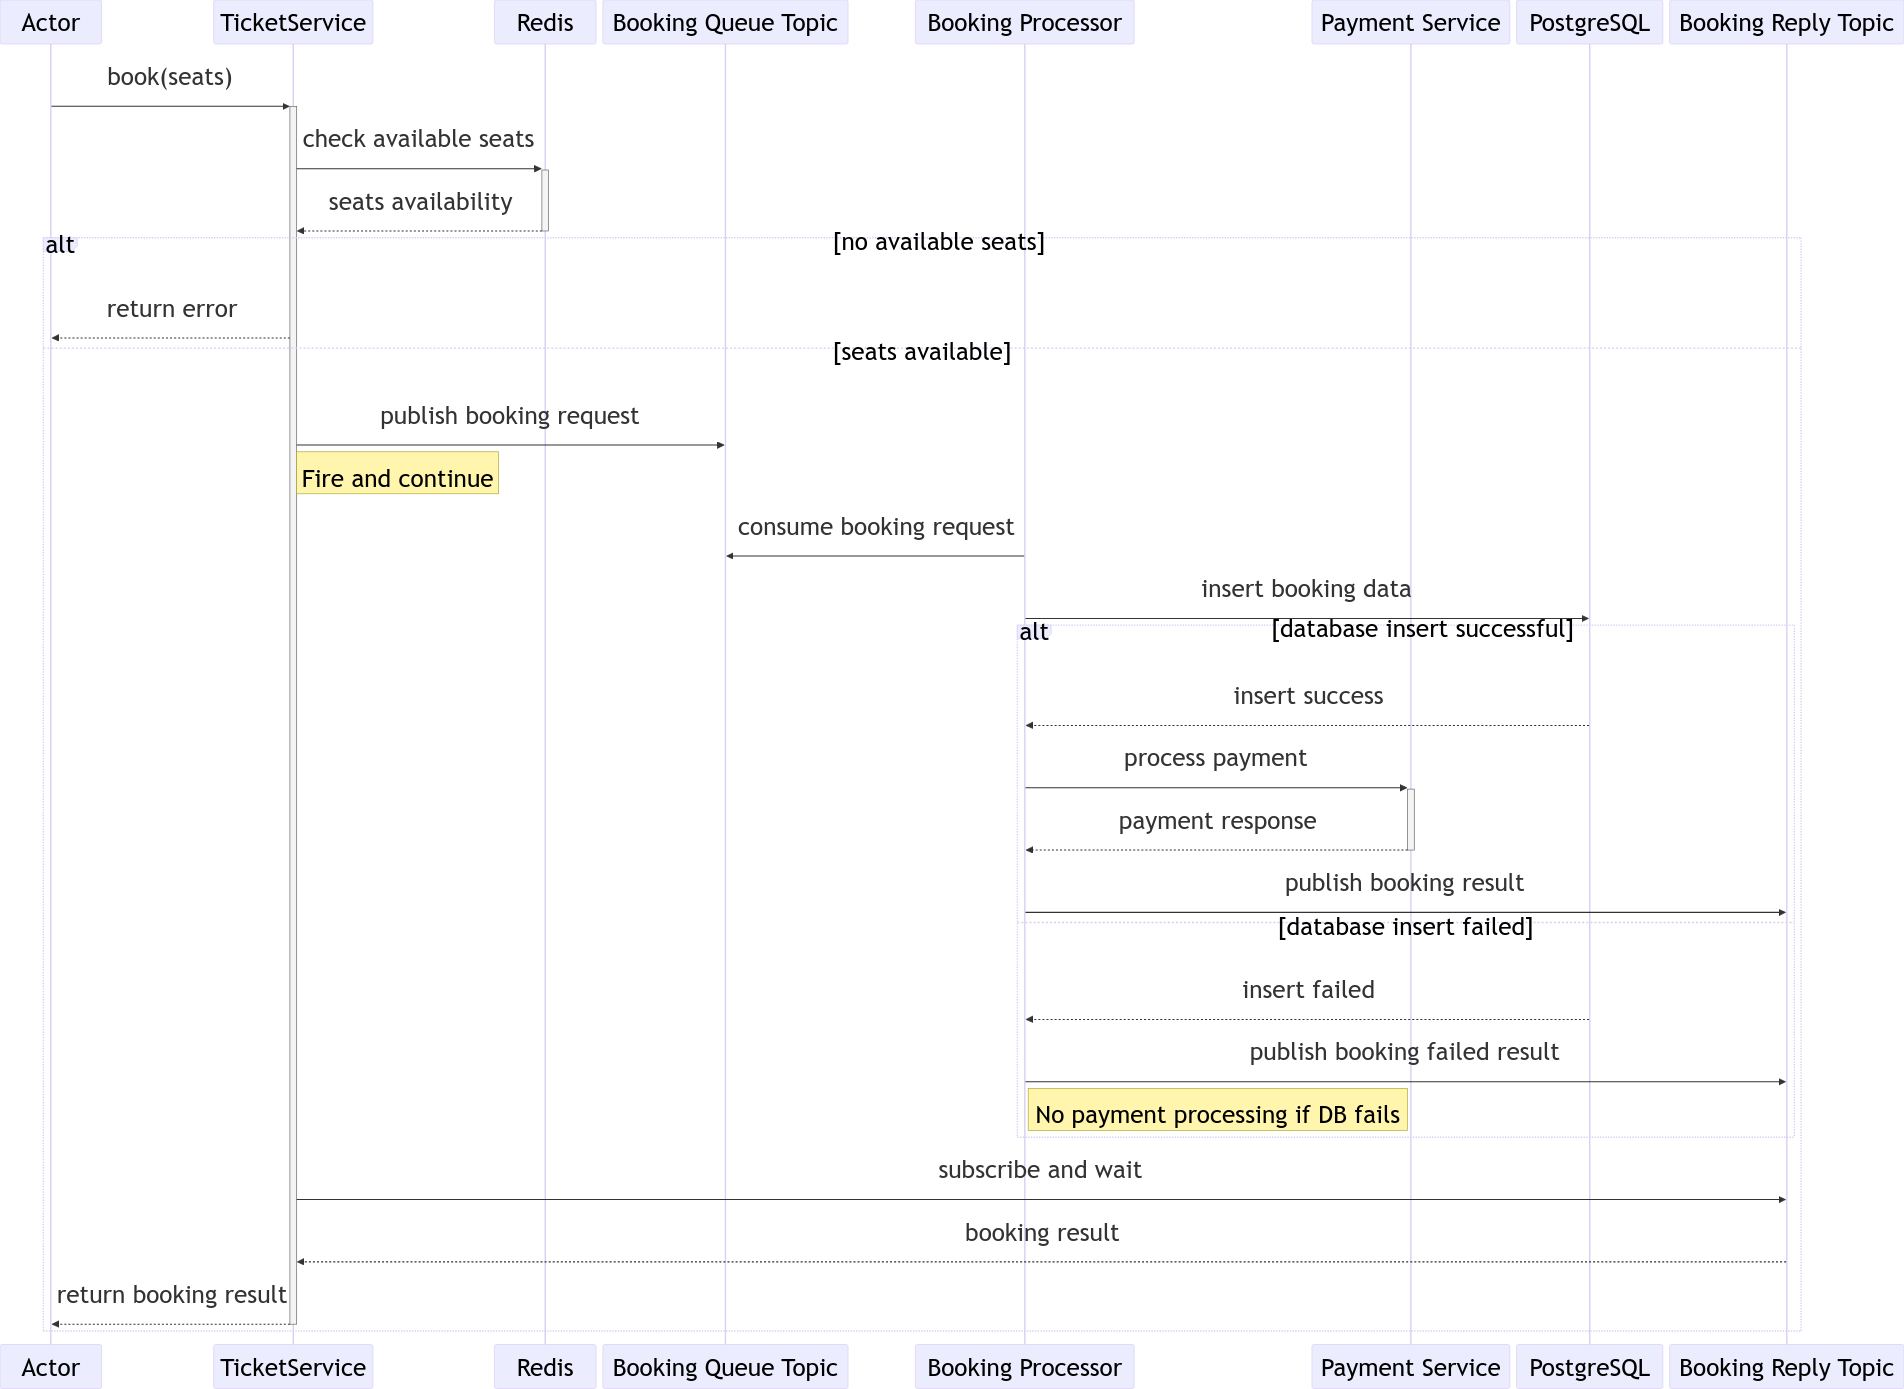
\includegraphics[width=1\textwidth]{resources/appendix/pgp-purchase-flow.png}
    \caption{Alur Pemesanan Tiket}
    \label{fig:pgp-purchase-flow}
\end{figure}

Terdapat dua isu yang harus dibahas pada pendekatan ini, yaitu:

\begin{enumerate}
    \item \textit{Persistence} pada Redis bersifat asinkron, sehingga terdapat kemungkinan data hilang ketika terjadi kegagalan. Meskipun begitu, penggunaan \textit{key-value store} lain yang \textit{persistent} berpotensi memperlambat kinerja. Dalam kasus ini, Redis akan dikonfigurasikan dalam mode kluster untuk penskalaan secara horizontal dan kombinasi antara \textit{snapshot} dan AOF untuk \textit{persistence}. Hilangnya data dapat terjadi ketika terdapat \textit{node} yang mengalami kegagalan. Meskipun begitu, \textit{data loss} atau \textit{eventual consistency} tidak akan mengganggu integritas sistem karena masih akan ada validasi lagi ketika pemrosesan pesanan.
    \item Isu \textit{fairness} harus diperhatikan ketika menggunakan Redpanda sebagai antrean. Redpanda hanya menjamin \textit{ordering} dalam satu partisi yang sama dan tidak menjamin \textit{ordering} secara global dalam satu topik. Salah satu cara untuk memastikan \textit{fairness} adalah dengan melakukan pembagian/ pemartisian antrean berdasarkan kategori tiket. Dengan begitu, pemrosesan pada antrean akan sesuai dengan urutan permintaan. Meskipun begitu, pendekatan ini mengharuskan pembelian lebih dari satu tiket dalam satu waktu hanya mendukung pemesanan dalam satu kategori yang sama.
\end{enumerate}

\subsubsection{Pelimpahan Tanggung Jawab Baca Kepada RisingWave}

Arsitektur ini mengoptimalkan sistem dengan pola CQRS. Tanggung jawab permintaan baca dilimpahkan kepada RisingWave. \textit{Streaming database} ini mengonsumsi \textit{CDC stream} dari kluster PostgreSQL, lalu memperbarui kueri secara inkremental. Hal yang perlu diperhatikan dalam penggunaan RisingWave adalah \textit{replication lag}. Data yang dikembalikan oleh RisingWave tidak valid apabila data tersebut \textit{outdated}.

\subsubsection{Penskalaan Pada PGP}

Scaling citus ya tambah instance. Redpanda dapat dibuat kluster dengan pemartisian data untuk meningkatkan \textit{throughput}.